\documentclass{article}
\usepackage[latin1]{inputenc}
\usepackage{enumerate}
\usepackage{hyperref}
\usepackage{graphics}
\usepackage{graphicx}
\usepackage{caption}
\usepackage{subcaption}
\usepackage{tabularx}
\usepackage{amsmath}
\usepackage{mathtools}

\usepackage{siunitx}
\usepackage{mhchem}

\newcommand{\ket}[1]{\ensuremath{\left|#1\right\rangle}}
\newcommand{\bra}[1]{\ensuremath{\left\langle#1\right|}}
\newcommand{\braket}[2]{\ensuremath{\left\langle #1 \middle| #2 \right\rangle}}
\newcommand{\obar}[1]{\ensuremath{\overline{ #1 }}}
% enumerate is numbered \begin{enumerate}[(I)] is cap roman in parens
% itemize is bulleted \begin{itemize}
% subfigures:
% \begin{subfigure}[b]{0.5\textwidth} \includegraphics{asdf.jpg} \caption{} \label{subfig:asdf} \end{subfigure}
\hypersetup{colorlinks=true, urlcolor=blue, linkcolor=blue, citecolor=red}
\graphicspath{ {C:/Users/Evan/Desktop/} }
\title{Final Projects}
\author{PHY 110C\\Evan Ott}
%\date{DATE}
\setcounter{secnumdepth}{2}
\usepackage[parfill]{parskip}
\begin{document}
\maketitle

For your final project, you will need to combine the data analysis and typesetting skills you've used all semester. You will select one of the projects below, then send us the completed
\LaTeX~and \textit{Mathematica} files. As always, send it to \href{mailto:data.analysis.physics@gmail.com}{data.analysis.physics@gmail.com}. The write-up should be a
(semi-)formal report on how you did what you did. We want to see the math you used, some graphs / tables that help explain what you're analyzing, and a little about
the \textit{Mathematica} constructs used. You don't need to tell us about basic things like using a \texttt{Table}, but if you had a difficult integral or
used a built-in distribution, you can mention it. We're focused on the data analysis, so you don't need to include historical context, much lab setup (in the case of a Modern Lab
report), etc. This is our way of determining if you have mastered the coursework over the course of the semester, so don't hold back on showing off.

\section{Home Field Advantage}
For this project, you will investigate the truth behind the ``Home Field (Court, etc.) Advantage:'' professional teams tend to win during games played in their local
stadium. The data for this project were condensed from play-by-play data from
Basketball Geek \cite{basketballgeek}, selecting all games from the 2008-2009 NBA season (excluding those that went into overtime) for a total of 1125 games. The format of the data is in Table \ref{tab:data}.
The data is on the assignment page of the online textbook.

Complete the sections outlined below, then write up results in a \LaTeX~document. Be sure to include some figures, tables, equations, or other structures.

\begin{table}
\begin{center}
\begin{tabular}{*{10}{|c}|}
Home& Q1$_H$&Q2$_H$&Q3$_H$&Q4$_H$&Away&Q1$_A$&Q2$_A$&Q3$_A$&Q4$_A$\\
\hline
BOS&20&14&19&16&CLE&19&12&13&17\\
CHI&19&14&22&20&MIL&25&18&19&18\\
\multicolumn{10}{|c|}{$\vdots$}
\end{tabular}
\caption{Representation of data set. Numerical values are number of points scored \textit{in the quarter} (QX$_H$ is points scored by home team, QX$_A$ is for the away team). Each row is a
different game. Included are the abbreviations for the teams. }
\label{tab:data}
\end{center}
\end{table}

\subsection{Game Results}
\label{sec:results}
To investigate the Home Field Advantage, we first need to see if such an effect is present in the data at the end of the game. Calculate the difference in score at the end of each game
(scores from each quarter add, in case you aren't the sports type). If a Normal (Gaussian) distribution seems appropriate for the data, fit the mean $\mu$ and standard deviation $\sigma$
of the score difference at the end of the game. Based on the mean, is there an advantage to playing at home? Based on the mean and spread of the data, how often should we
expect a home team to win (using no information about player stats, etc.)? Show visually that the data agrees with a Normal distribution by overlaying a probability
density function histogram and probability density function of the fitted Normal distribution (something similar to Figure \ref{fig:normal}).

\begin{figure}
\begin{center}
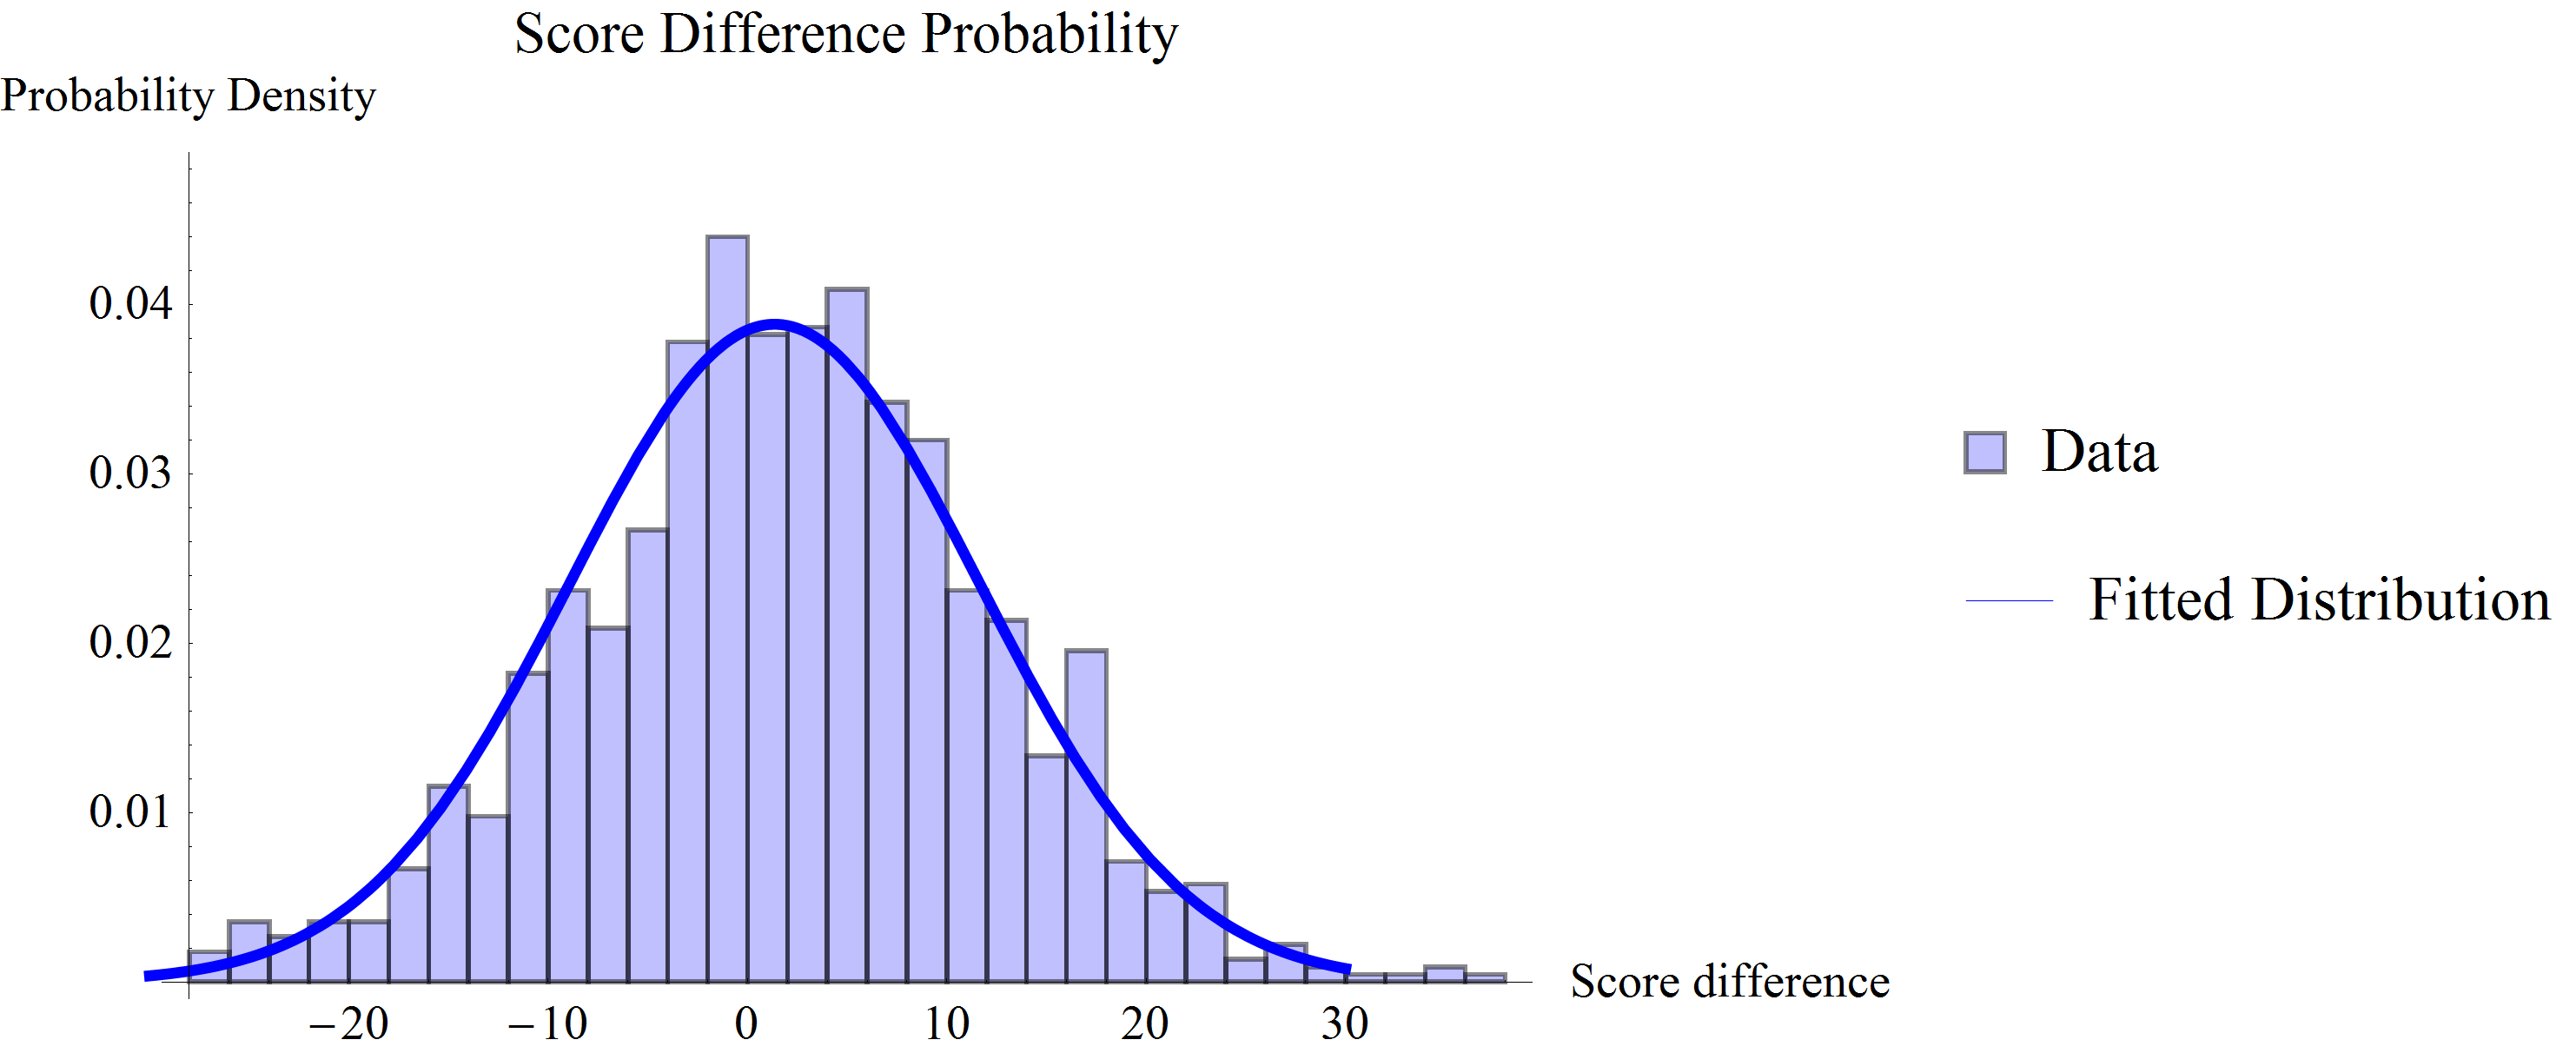
\includegraphics[scale=.7]{normalfit.png}
\caption{Example graphic indicating data and fitted normal distribution.}
\label{fig:normal}
\end{center}
\end{figure}

\subsection{In-Game Progression}
\label{sec:progression}
Now, let's characterize how the point difference changes throughout a game (on average). If we make the assumption that the play in each quarter is independent
(first quarter performance has no bearing on fourth quarter, etc.), then we should expect the general properties of adding independent Normally-distributed variables:
\begin{itemize}
\item{Taking $\mathcal{N}(\mu_1,\sigma_1)\pm\mathcal{N}(\mu_2,\sigma_2)$ gives a combined mean of $\mu=\mu_1\pm\mu_2$.}
\item{Taking $\mathcal{N}(\mu_1,\sigma_1)\pm\mathcal{N}(\mu_2,\sigma_2)$ gives a combined variance of $\sigma^2=\sigma_1^2+\sigma_2^2$ (variances \textit{always} add).}
\end{itemize}
Let's also assume (for the moment -- we'll test it momentarily) that each quarter is approximately the same ($\mu_1\approx\mu_2$, $\sigma_1\approx\sigma_2$, etc.).

From this, can you come up with a model for
the mean difference in score as a function of percentage of time played so far during a game? For the standard deviation of the difference in score as a function
of percentage of time played so far during a game? This creates functions $\mu(t)$ and $\sigma(t)$ where $t\in[0,1]$. We know the final score and spread from subsection~\ref{sec:results} ,
and we know the initial score and spread as well (starts at 0--0 with $\sigma=0$). In your report, please discuss how you arrived at the functions you did.

\textit{Hint:} $\mu(t)$ and $\sigma(t)$ should have the boundary properties outlined above: 
\begin{itemize}
\item{$\mu(0)=0$}
\item{$\sigma(0)=0$}
\item{$\mu(1)=\mu=\mu_1+\mu_2+\mu_3+\mu_4$}
\item{$\sigma^2(1)=\sigma^2=\sigma_1^2+\sigma_2^2+\sigma_3^2+\sigma_4^2$}
\end{itemize}
then also be able to predict the distribution at half-time ($\mu(.5)=\mu_1+\mu_2$, and $\sigma^2(.5)=\sigma_1^2+\sigma_2^2$). If this part stumps you, feel free to ask your student teachers about it.

\subsection{Model-Fitting Game Progression}
\label{sec:model}
With the model for $\mu(t),~\sigma(t)$ from subsection \ref{sec:progression}, use a \texttt{LinearModelFit} or \texttt{NonlinearModelFit} in \textit{Mathematica}
to fit the coefficient based on the data at each quarter (rather than just using the final distribution). For example, you'll have \textit{Mathematica} fit the function
$\mu(t)$ to the data:
$$\{\{0,~0\},~\{0.25,~\mu_1\},~\{0.5,~\mu_1+\mu_2\}~\{0.75,~\mu_1+\mu_2+\mu_3\},~\{1,~\mu_1+\mu_2+\mu_3+\mu_4\}\}$$
These fitting functions provide the estimate of the parameter \textit{and} the standard error in the parameter (use the 
``\texttt{ParameterTable}'' field of the fit -- see the documentation) along with the $p$-value. 

The $p$-value reported is the probability of getting an estimated
coefficient this far from $0$ if there is no dependence on the coefficient. For example, a $p$-value of $0.9$ says that $90\%$ of the time, we would fit a coefficient
this different from 0 where there really is no dependence. Based on the reported $p$-values, was the fit sufficient?

If so, using the estimate and error for the mean vs. time and for the standard deviation vs. time,
is the model based only on final scores consistent with the fitted data? More formally, are the coefficients used in the simple model from subsection \ref{sec:progression} consistent
with those determined by the fits in this subsection? How many ``standard errors'' away from each other are they? Is the difference statistically significant at the 
$99\%$ confidence level (i.e., should we be
surprised at the result from the simple model if it is indeed drawn from the one we fitted)?

\subsection{Results}
Using results from subsection \ref{sec:model}, present a visual indicating how all the games compare with the average and standard deviation of the distribution at the end of each quarter. You
may want to use the \texttt{ErrorListPlots} module in \textit{Mathematica}. Feel free to explore different representations and include them in your submitted \textit{Mathematica} document.

\subsection{Bonus: Single-Game Predictions}
Does the Home Field Advantage work for a specific team? Select a team and use a variation of the techniques above to determine if they are more likely to win home games or away games.

\subsection{Bonus: Working with Normal Distributions}
Using the same ``independence'' approximations above, find the actual score at half-time for a few games, then predict the probability the team should win assuming the
game is representative. In other words, based on $\mu_{3-4}=\mu_3+\mu_4,~\sigma_{3-4}^2=\sigma_3^2+\sigma_4^2$ and $\mu_{f}=D_2+\mu_{3-4},~\sigma_f=\sigma_{3-4}$ (with
$D_2$ being the score difference at half-time), determine what certainty you have that the home team will win the game. 

\section{Hubble Constant}
Details to come.

\section{Modern Lab}
Details to come.

\begin{thebibliography}{9}
\bibitem{basketballgeek} \url{http://www.basketballgeek.com/downloads/2008-2009.regular_season.zip}
\end{thebibliography}

\end{document}